\section{从单项到组合：改进方案的选择}
\label{sec:selection}

\subsection{分别检查两项过滤调整的作用}
初轮结果支持放宽短段过滤，但最终设置同时改变了点数与长度条件。若不拆开比较，就无法判断收益来自哪一项，也无法确认二者是否都需要保留。因此，在240条已观察记录、23,950个原始点上，分别降低最少点数、取消长度下限，再检查联合调整。

表\ref{tab:development}保留各单项与组合的完整结果。“过滤调整”指最少点数2、最短长度0，其余仍为参考。方向60与DP2、DP10是相应单项，组合只在已有对照上加入指定变化，不同时更换坐标、数据或评价目标。

\begin{table}[htbp]\centering\small
\caption{240条开发记录上的单项与组合。比较参考为相同的原始设置}\label{tab:development}
\begin{tabularx}{\linewidth}{@{}Yrrrrr@{}}\toprule
方案 & 共同覆盖 & 保留点 & D删除 & 保护失败 & 严格改善\\\midrule
参考设置 & 17,213 & 5,349 & 1,427 & 0 & 0\\
仅点数降至2 & 17,379 & 5,479 & 1,427 & 0 & 30\\
仅长度下限为0 & 23,706 & 5,590 & 1,540 & 0 & 77\\
过滤调整 & 23,917 & 5,751 & 1,540 & 0 & 107\\
统一方向60度 & 17,213 & 5,591 & 605 & 3 & 97\\
DP容差2 & 17,213 & 7,295 & 1,427 & 9 & 60\\
DP容差10 & 17,213 & 3,869 & 1,427 & 173 & 0\\
方向条件规则 & 17,213 & 5,434 & 992 & 0 & 41\\
过滤＋方向条件 & 23,917 & 5,836 & 1,058 & 0 & 142\\
过滤＋DP2 & 23,917 & 7,761 & 1,540 & 9 & 149\\
过滤＋DP10 & 23,917 & 4,250 & 1,540 & 178 & 60\\\bottomrule
\end{tabularx}
\tabnote{失败和改善按记录计，均相对参考，二者不是互补计数；有部分改善不意味着全部保护通过。P单项还需在相同输入与共同误差预算下判断压缩收益，不能由本表的改善数直接选出。}
\end{table}

联合过滤调整使共同覆盖增加6,704点，107条记录有严格改善，无输出记录由65降到0。这一收益来自恢复覆盖，而不是在参考已覆盖范围内观察到统一的几何改善。只降低点数，少保留其中6,538个覆盖点；只取消长度下限，少保留211个覆盖点。因此，两项调整均对联合结果有独立作用，但不能把两个单项的改善数直接相加。

这里的较短片段仍可能包含重复位置或位置异常。接受过滤调整表示它减少了按参考条件整段舍弃的信息，后续仍需检查新增范围的偏差；不能将取消长度下限解释为所有短段都已证明有实际出行价值。

\clearpage
\subsection{方向条件规则能否提供额外收益}
统一放宽方向阈值到60度，在开发集上有3条共同几何保护失败，不能直接替换参考。但删除较少的影响可能与采样情况有关，因此进一步测试一个简单规则：若整条记录的原始相邻时间差均可计算，且全部满足$0<\Delta t\leq30$秒，使用60度；其余仍用35度。它只读取原始时间，不按记录编号匹配答案。

开发中满足与不满足该条件的记录各120条。单独使用这一规则，相对参考在41条记录上降低共同最大几何偏差，全部记录通过保护；但它没有恢复过滤调整新增的6,704个覆盖点。两项作用因此具有进一步组合的依据，而非仅因它们都曾出现好结果就直接相加。

“过滤＋方向条件”与参考、两个父方案分别比较。相对过滤调整，覆盖不变，41条几何改善，显式存储增加85点；相对仅方向条件，107条恢复覆盖。相对最初参考共有142条严格改善，是107条覆盖改善与41条几何改善的并集，二者交叠6条。

移去方向规则，失去41条已观察到的几何改善；移去过滤调整，则丢回6,704个覆盖点，使65条重新无输出。这使组合成为开发阶段暂时保留的方案。\textbf{开发中的支持仍需在新的记录上检验，不能直接作为最终采用理由。}

\subsection{DP组合没有因压缩更多而被直接采用}
DP2使即时误差更小，但需要更多输出点；DP10更省点，却可能越过共同预算。为识别P组件自身的作用，每个P变体都与\textbf{完全相同上游、容差为5}的方案比较。

\begin{table}[htbp]\centering\small
\caption{相同P输入上的容差调整：省点收益与误差约束分开判断}\label{tab:p-combination}
\begin{tabularx}{\linewidth}{@{}YrrY@{}}\toprule
比较 & 输出点变化 & 超5预算记录 & 取舍\\\midrule
参考上游：DP2对DP5 & +1,946 & 0 & 未带来压缩收益\\
参考上游：DP10对DP5 & $-1,480$ & 173 & 超出预算\\
过滤调整：DP2对DP5 & +2,010 & 0 & 未带来压缩收益\\
过滤调整：DP10对DP5 & $-1,501$ & 178 & 超出预算\\\bottomrule
\end{tabularx}
\end{table}

过滤与DP2组合虽有覆盖增加，但该增加已由S产生，不能归功于更紧的P容差；它还比相同上游多存2,010点。过滤与DP10则在178条记录上超出预算。两种组合都没有成为更合适的统一方案，较紧容差也不是完整原始几何必然逐点改善的保证。

组合比较增加了一个轻量方向规则及三个组合设置，并完成必要父项和移除检查。另一类删除保护缺少可靠的位移或物理阈值依据，没有为凑齐候选而加入。已有顺序、在线模式也没有新的支持机制，因而不继续无依据扩展。此时保留参考、过滤调整、方向条件及二者组合四个方案，进入独立的选择阶段。

\clearpage
\subsection{组合在新记录上退化之后，怎样取舍}
新选择集含240条记录、24,677点，四个方案在查看结果前已固定。过滤调整在全部记录上保持规定保护，103条共同覆盖严格增加，共增加6,625点。方向条件及其组合虽然仍改善部分记录，却在同三条记录上增大共同最大几何偏差。

\begin{table}[htbp]\centering\small
\caption{四个固定候选在新选择记录上的表现}\label{tab:selection}
\begin{tabularx}{\linewidth}{@{}Yrrrr@{}}\toprule
方案 & 共同覆盖 & 显式保留 & 保护失败 & 严格改善\\\midrule
参考设置 & 18,016 & 5,321 & 0 & 0\\
过滤调整 & 24,641 & 5,784 & 0 & 103\\
方向条件规则 & 18,016 & 5,360 & 3 & 39\\
过滤＋方向条件 & 24,641 & 5,823 & 3 & 138\\\bottomrule
\end{tabularx}
\tabnote{失败和严格改善均相对参考；组合相对过滤调整另有39条几何改善，但其他记录的收益不能抵消三条失败。}
\end{table}

\begin{figure}[H]\centering
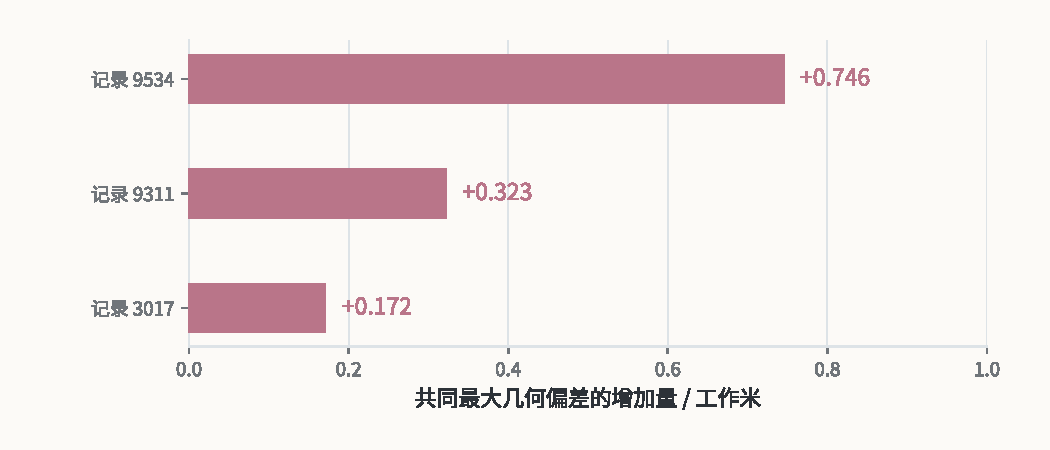
\includegraphics[width=.98\linewidth]{figures/selection_geometry_increase.pdf}
\caption{方向条件加入过滤调整后，三条选择记录的共同最大偏差增加。记录3017、9311、9534的原偏差分别为4.786、3.953、3.718工作米，组合后为4.957、4.276、4.464。图中展示差值，三条均未满足逐记录非退化条件。}\label{fig:selection}
\end{figure}

较宽方向阈值保留了更多点，随后同一个DP5算法在变化后的输入上重新选点。例如记录9311的最终点数仍为10，但原索引27被换为22，共同最大误差由3.953415增至4.276002工作米。两边的P即时误差均不超过5，所以不是DP实现违反定义，而是合法处理后出现真实权衡。

因此，实验没有修改分组条件，也没有从选择集删去这三条记录，而是去掉方向条件，保留较简单的过滤调整。最终仍为S-D-P：时间30秒、距离400工作米、最少2点、最短长度0、方向35度、DP容差5工作米。该决定依据已有比较；下一章再检查其在预留记录上的表现及全量结果。
